\section{Barrier methods} \label{section_71}

In this chapter, we look into barrier methods as an alternative for solving linear programming problems. Barrier methods stem from early developments of methods for solving constrained nonlinear programming problems which had as main characteristic the \emph{strict} satisfaction of the constraints throughout the method. Because of this feature, these methods became generally known as interior point methods. This is however not the case anymore, and most implementations of interior point methods benefit from features that allow the search to ``leave the interior'' of the feasible region. Hence, it became common to refer to these methods with the more general name of barrier methods.

A subclass of barrier methods called \emph{primal-dual methods} distinguishes itself as an efficient method, with practical performance surpassing in many cases that of the simplex method. Currently, most professional-grade solvers have built-in implementations of barrier methods.

In essence, barrier methods are the method of choice of many nonlinear \emph{local solver}, which are targeted towards nonlinear optimisation problems. The term local refers to the fact that solutions found can only be guaranteed to be locally optimal. Of course, for convex optimisation problems, this is not an issue, as a local solution is globally optimal.

In general, the simplex methods often perform better in small and medium problems, whilst barrier methods typically perform better on large-scale problems. This is largely because, as we will see, the main operation in a barrier method is the solution of (large) linear systems of equations, which can be done rather efficiently and in ways that explore the structure of the problem (e.g., matrix sparsity can be exploited by factorisation techniques) to reap computational performance improvements.


\section{Newton's method with equality constraints} 


In essence, barrier methods consist of the employment of a variant of Newton's method to solve the optimality conditions of optimisation problems. In the context of linear programming problems, this is equivalent to finding solutions that are both primal and dual feasible.

We consider a version of Newton's method called the Newton-Raphson (NR) method, which was originally designed for finding roots of vector functions. Let $f: \reals^n \to \reals^n$, with $f_i : \reals^n \to \reals$ differentiable for $i = 1,\dots,n$.

We wish to find a solution $x^*$ that is a root for $f$, i.e., $f(x^*) = 0$. For that, we must solve the system of equations given by
	$$ 
	f(x) = \begin{bmatrix} f_1(x) \\ \vdots \\ f_n(x) \end{bmatrix} = \begin{bmatrix} 0 \\ \vdots \\ 0 \end{bmatrix}.
	$$
	
The NR method starts from an initial guess $x^k$ for $x^*$ and iterates by finding the root for a \emph{linear} (i.e., first-order Taylor) approximation of $f$ at $x^k$. Under suitable conditions, including having a starting point $x^0$ that is within a neighbourhood of the root of $f$, the sequence $\braces{x^k}_{k\to\infty}$ converges to $x^*$.

Let us clearly state how the method iterates. At a given $x^k$, the first-order approximation of $f(x)$ is given by
	$$ 
	f(x^k + d) = f(x^k) + \nabla f(x^k)^\top d,
	$$
	where $\nabla f(x^k)$ is the \emph{Jacobian} of $f(x)$, which is defined as
	$$ 
	\nabla f(x^k) = \begin{bmatrix} \nabla f_1(x^k)^\top \\ \vdots \\ \nabla f_n(x^k)^\top \end{bmatrix}. 
	$$
	
The algorithm proceeds by finding the step to be taken from $x^k$ to reach the root of the first-order approximation of $f$ at $x^k$. This means that we want to obtain $d$ such it solves the first-order approximation of $f(x^k + d) = 0$. Thus, we must solve
	%
	\begin{equation*}
		f(x^k) + \nabla f(x^k)^\top d = 0 \Rightarrow
		d = -\nabla f(x^k)^{-1}f(x^k).
	\end{equation*}
	
Consider the following numerical example. Suppose we would like to find the root of $f$ with $x^0 = (1,0,1)$, where $f$ is given by 
	$$
	f(x) = \begin{bmatrix}f_1(x) \\ f_2(x) \\ f_3(x) \end{bmatrix} = \begin{bmatrix} x_1^2 + x_2^2 + x_3^2 -3 \\ x_1^2 + x_2^2 - x_3 - 1 \\ x_1 + x_2 + x_3 - 3 \end{bmatrix}
	$$
	The Jacobian of $f$ is given by 
	$$
	\nabla f(x)=\begin{bmatrix} 2x_1 & 2x_2 & 2x_3 \\ 2x_1 & 2x_2 & -1 \\ 1 & 1 & 1\end{bmatrix}.
	$$
	
	The algorithm starts by calculating $d^0$, which is given by
	$$
	d^0 = -[\nabla f(x^0)]^{-1}f(x^0) = - \begin{bmatrix} 2 & 0 & 2 \\ 2 & 0 & -1 \\ 1 & 1 & 1\end{bmatrix}^{-1}\begin{bmatrix} -1 \\ -1 \\ -1 \end{bmatrix} = \begin{bmatrix} 1/2 \\ 1/2 \\ 0 \end{bmatrix}.
	$$ 
	%
	Thus, the first point is 
	$$
	x^1 = x^0 + d^0 = \begin{bmatrix} 3/2 & 1/2 & 1\end{bmatrix}.
	$$ 
	%
	To infer that the method has converged, we can either check whether $f(x^k) \approx 0$ or whether if $||x^{k+1} - x^{k}||_2 = || d^{k} ||_2 \approx 0$. As $||x^1 - x^0||_2 = || d^0 ||_2 \approx 0.7$, the method carries on until we find that $|| d^k|| < \epsilon$. If we adopt a numerical tolerance of $\epsilon = 0.01$, meaning that any number below this threshold is deemed acceptably close to zero, then $x^* = (1, 1, 1)$ is reached after approximately 20 iterations.	

\section{Interior point methods linear programming problems}
	
We start by focusing on the primal-dual interior point method, as originally proposed. Then, we will focus on the modifications that turn it capable of iterating through some not necessarily interior solutions in a strict sense. 	

We start by considering our linear programming problem in standard form 
	\begin{align*}
		(P) :~ \mini \ &c^\top x \\
		\st &Ax = b,  \\
		&x \ge 0 
	\end{align*}
	%
	and its associated dual, which is stated as
	%
	\begin{align*}
		(D) :~ \maxi \ &b^\top p \\
		\st &A^\top p + u = c, \\
		&u \ge 0. 
	\end{align*}
	%
	Notice that the dual is also posed in a form where the inequalities (originally $A^\top p \le c$) are converted to equalities requiring the additional variable $u$. An alternative way to think about $u$ is as it were the dual variable associated with the nonnegativity constraints $x \ge 0$. 
	
Recall that the optimality conditions for problem $P$ can be expressed as
	%
	\begin{align} 
		& Ax = b, \ \ x \ge 0, \label{p1c7:eq:optimality_conditions_primal} \\
		& A^\top p + u = c, \ \ u \ge 0, \label{p1c7:eq:optimality_conditions_dual} \\
		& u^\top x = 0. \label{p1c7:eq:optimality_conditions_cc}  
	\end{align}
	%
	The first two conditions are primal \eqref{p1c7:eq:optimality_conditions_primal} and dual \eqref{p1c7:eq:optimality_conditions_dual} feasibility conditions, while \eqref{p1c7:eq:optimality_conditions_cc} is an alternative way of stating complementarity conditions on the nonnegativity constraints $x \ge 0$.
	
One initial idea could be simply, from a purely methodological standpoint, to employ NR to solve the above system of equations. The caveat, however, is that one must observe and retain the nonnegativity conditions $x > 0$ and $s >0$, which are an important complicating factor in this setting. Indeed, one could, departing from a feasible solution $(x,p,u)$, employ NR to find a solution for \eqref{p1c7:eq:optimality_conditions_primal}-\eqref{p1c7:eq:optimality_conditions_cc} while controlling the steps taken using each Newton direction such that the nonnegativity conditions $x > 0$ and $s >0$ are retained, in a similar fashion to how it is done in the simplex method. However, it turns out that Newton directions obtained from successive iterations considering \eqref{p1c7:eq:optimality_conditions_primal}- \eqref{p1c7:eq:optimality_conditions_cc} typically require considerably small steps to be taken such that the nonnegativity conditions are retained, which renders the algorithm less useful from a practical standpoint.
	   
	
This is precisely when the notion of an interior solution plays a role. An \emph{interior point} is defined as a point that satisfies primal feasibility conditions strictly, that is $Ax = b$ with $x > 0$, and has also $s >0$, implying that the complementarity conditions \eqref{p1c7:eq:optimality_conditions_cc} are \emph{violated}. This notion of interior points is useful in that it allows for the definition of less ``aggressive'' Newton directions, which aim towards directions that instead can reduce the amount of violation in the complementarity conditions. Thus, we can alternatively consider the system with \emph{relaxed} complementarity conditions 	
	%
	\begin{align*}
		& Ax = b, \ \ x \geq 0,\\ 
		& A^\top p + u = c, \ \ u \geq 0, \\
		& u_j x_j = \mu, \ \forall j \in J 
	\end{align*}
	%
	to provide Newton directions, while, simultaneously, gradually making $\mu \to 0$. By doing so, one can obtain not only directions which can be explored with larger step sizes, thus making more progress per iteration but also yield methods with better numerical properties.
	
To see how that can be made operational, let us first define some helpful notation. Let $X\in \reals^{n\times n}$ and $U \in \reals^{n \times n}$ be defined as
	%
	$$
	X = \diag(x) = \begin{bmatrix} \ddots & & \\   
	                                        & x_i & \\
	                                        & & \ddots     
	                 \end{bmatrix}
	                 \text{ and }
	U = \diag(u) = \begin{bmatrix} \ddots & & \\   
	                                        & u_i & \\
	                                        & & \ddots     
	                 \end{bmatrix}               
	$$
	%
	and let $e = [1,\dots,1]^\top$ be a vector of ones of suitable dimension. We can rewrite the optimality conditions \eqref{p1c7:eq:optimality_conditions_primal}- \eqref{p1c7:eq:optimality_conditions_cc} in matrix form as 
	%
	\begin{align*}
		&Ax = b, \ x > 0, \\ 
		&A^\top p + u = c, \ u > 0,\\ 
		&XUe = 0, 
	\end{align*}
	%
 	and, analogously, state their relaxed version (i.e., with relaxed complementarity conditions) as
 	%
 	\begin{align}
		&Ax = b, \ x > 0, \label{p1c7:eq:optimality_conditions_matrix_primal}\\ 
		&A^\top p + u = c, \ u > 0, \label{p1c7:eq:optimality_conditions_matrix_dual}\\ 
		&XUe = \mu e. \label{p1c7:eq:optimality_conditions_matrix_relaxed_cc}
	\end{align}

We start from a feasible solution $(x^{k}, u^{k}, p^{k})$. We can then employ NR to solve the system \eqref{p1c7:eq:optimality_conditions_matrix_primal}-\eqref{p1c7:eq:optimality_conditions_matrix_relaxed_cc} for a given value of $\mu$. That amounts to finding the Newton direction $d$ that solves $f(x^k) + \nabla f(x^k)^\top d = 0$, in which
	%
	\begin{equation*}
	f(x^k) = \begin{bmatrix}
				Ax^k - b \\
				A^\top p^k + u^k - c \\
				X^k U^k e - \mu e 
			   \end{bmatrix},	   
		\ \nabla f(x^k) = \begin{bmatrix}
					   A & 0 & 0 \\
					   0 & A^\top & I \\
					   U^k & 0 & X^k	
					  \end{bmatrix}
		 \text{ and } d = (d_x^k, d_p^k, d_u^k) = 
			\begin{bmatrix}
			x - x^k \\ 
			p - p^k \\
			u - u^k
		\end{bmatrix}.
	\end{equation*}	
	
Once the direction $d^k = (d_x^k, d_p^k, d_u^k)$ is obtained, we must calculate step sizes that can be taken in the direction $d^k$ that also retain feasibility conditions, meaning that they do not violate $x >0$ and $u > 0$ at the new point. One simple idea is to follow the same procedure as the simplex method. That is, let $\theta_p^k$ and $\theta_d^k$ be the iteration $k$ step sizes for $x$ and $(p,u)$, respectively. Then they can be set as
	%
	\begin{equation*}
		\theta_p^k = \min_{i:d_{x_i}^k < 0} - \frac{x_i^k}{d_{x_i}^k} \text{ and }	\theta_d^k = \min_{i:d_{u_i}^k < 0} - \frac{u_i^k}{d_{u_i}^k},
	\end{equation*}
		%
		where $d_{x_i}^k$ and $d_{u_i}$ are the $i$-th component of the vectors $d_x^k$ and $d_u^k$, respectively, and $i = 1, \dots, n$. In practice, there are alternative, and arguably more efficient, ways to set step sizes, but they all are such that their maximum sizes are $\theta_p$ and $\theta_d$ as above and always strictly smaller than one (notice that our constraints are such that $x$ and $u$ are strictly positive).
		
		Once we calculated appropriate step sizes, we can then make 
		$$
		(x^{k+1}, p^{k+1}, u^{k+1}) = (x^{k} + \theta_{p}^kd_x^k, p^{k} + \theta_d^k d_p^{k}, u^{k} + \theta_d^k d_u^k).
	$$
	Then, we proceed by updating $\mu$ as $\mu = \beta \mu$, with $\beta \in (0,1)$ and repeat the same procedure until convergence, i.e., until $\mu$ is sufficiently small.  
		
Before discussing in more detail the practicalities of the method, let us take an alternative perspective on showing how the notion of interior plays a role in the design of the algorithm, which requires us to consider the notion of barrier functions. This will also serve as a justification for the name ``barrier methods''. 
	
	
\section{Barrier methods for linear programming problems}


Barrier methods are a class of optimisation methods designed to handle inequality-constrained problems of the form
	%
	\begin{align*}
	(P) : \mini \ & f(x) \\
	\st & g_i(x) \leq 0, \ i = 1,\dots,m \\
	& Ax = b. 
	\end{align*}
	%
	These methods use the notion of \emph{barrier functions} to remove inequality constraints and have them represented implicitly as an objective function term. This in turn allows for the use of NR as an underpinning numerical method. 
	
To see how it works, we can think of a barrier function as a surrogate for a feasibility indicator function $I$ that reacts to infeasibility in $g_i(x) \leq 0$, $\forall i \in  \braces{1,\dots, m}$. That is, $I : \reals \to \reals$ is such that
	%
	\begin{equation*}
	I(u) = \begin{cases} 0, &\text{if } u \leq 0 \\
	                     \infty, &\text{if } u > 0.  
	       \end{cases}
	\end{equation*} 

With that definition for $I$ at hand, we can then reformulate our problem as	
	%
	\begin{align*}
		\mini \ & f(x) + \sum_{i=1}^m I(g_i(x)) \\
		\st &Ax = b. 
	\end{align*}
	
The issue however is that $I$ is not numerically favourable, due to its nature of ``shooting to infinity'' (including the discontinuity it creates) whenever a solution $x$ is infeasible to the original problem. To circumvent that, we can use barrier functions instead, which are chosen to mimic the behaviour of $I$, whilst retaining more favourable numerical properties. The most widespread choice for barrier functions is the logarithmic barrier, which is given by
	%
	\begin{equation*}
		B_\mu(u) = -\mu \ln(-u)
	\end{equation*}
	%
	where $\mu > 0$ sets the accuracy of the barrier term $B_\mu(u)$. Figure \ref{p1c7:fig:barrier_function} illustrates the influence of $\mu$ in the shape of the barrier function for the unidimensional case. Notice how, as $\mu$ decreases, the logarithmic barrier more closely resembles the indicator function $I$.
	
\begin{figure}
	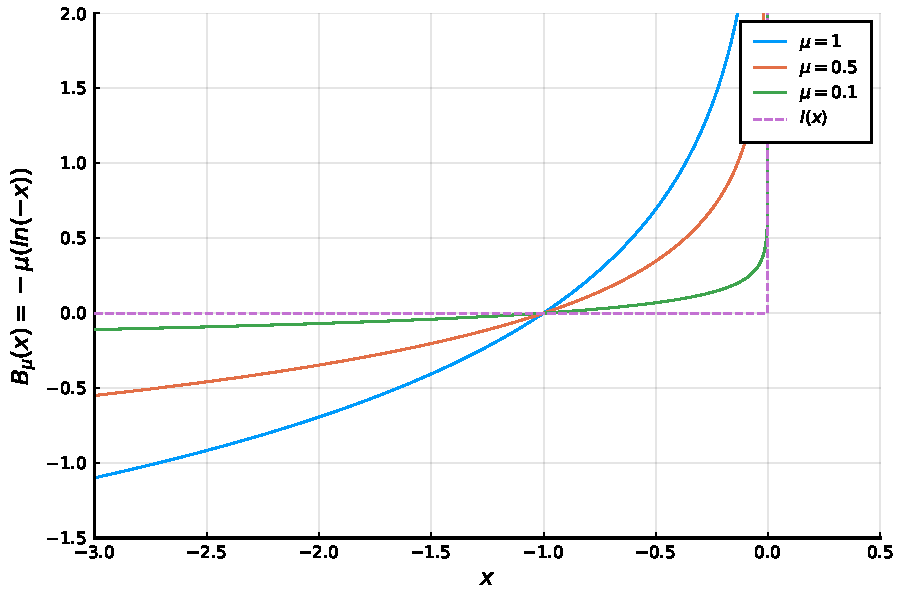
\includegraphics[width=0.8\textwidth]{part_1/chapter_7/figures/different_mu.pdf}
	\caption{Alternative barrier functions for different values of $\mu$. The dashed line represents the indicator function $I$ going to infinity when $u > 0$} \label{p1c7:fig:barrier_function}
\end{figure}

Using $B_\mu$ as the barrier function, the \emph{barrier problem} $P_\mu$ can be formulated as
	%
	\begin{align*}
		(P_\mu) : \mini \ &f(x) - \mu \sum_{i=1}^m\ln(-g_i(x)) \\
		\st & Ax = b.
	\end{align*}
	%
	This formulation has a number of important benefits. First, notice how this problem is such that, if one were to apply NR to solve its optimality conditions, one would be faced with solving linear systems of equations, regardless of the nature of the constraints $g_i(x) \le 0$, $i = 1,\dots, m$ (recall that NR solves first-order approximations of the original system of equations). This creates a bridge between linear algebra techniques and a wide range of nonlinear optimisation problems. 
	
Moreover, as discussed earlier, one can here also gradually decrease $\mu$ by making $\mu^{k+1} = \beta\mu$ with $\beta \in (0,1)$. This method is an idea generally known as Sequential Unconstrained Minimisation Technique (SUMT).As one may suspect, as $\mu \rightarrow 0$, we have that $x^*(\mu) \rightarrow x^*$, where $x^*(\mu)$ and $x^*$ are the optimal values for problems $P_\mu$ and $P$, respectively. However, for small values of $\mu$, the barrier problem becomes challenging numerically., which does not come as a surprise as the barrier resembles more and more the indicator function $I$ and all its associated numerical issues. 

Let us illustrate the above with an example. Consider the nonlinear problem 
	$$
	P : \mini \braces{f(x) = (x + 1)^2 : x \geq 0}.
	$$ 
	Notice that the unconstrained optimum would be $x =-1$ but the constrained optimum is $x^* = 0$. For this example, the barrier problem $P_\mu$ is
	%
	$$P_\mu : \mini f(x) + B_\mu(x) = (x + 1)^2 - \mu \ln(x).$$
	%
	Because this is a univariate convex function, we know that the optimum is attained where $(f(x) + B_\mu(x))' =0$. Thus, we have that
	%
	\begin{align*}
		& f^{~\prime}(x) + B_\mu^\prime(x) = 0 \\
		& 2(x+1) - \frac{\mu}{x} = 2x^2 + 2x -\mu = 0.
	\end{align*}
	%
	The positive solution (since we must have that $x > 0$) of $2x^2 + 2x -\mu = 0$ is given by
	$$ x^*(\mu) = \frac{-2 + \sqrt{4 + 8\mu}}{4}.  
	$$ 
	Notice that $\lim_{\mu \rightarrow 0}x^*(\mu) = 0$, which is indeed the optimal $x^*$ for $P$. Figure \ref{p1c7:fig:example-barrier} plots the function $f(x) + B_\mu(x)$ for alternative values of $\mu$ indicating their minima (found by substituting the value of $\mu$ in the expression for $x^*(\mu)$). 

\begin{figure}
	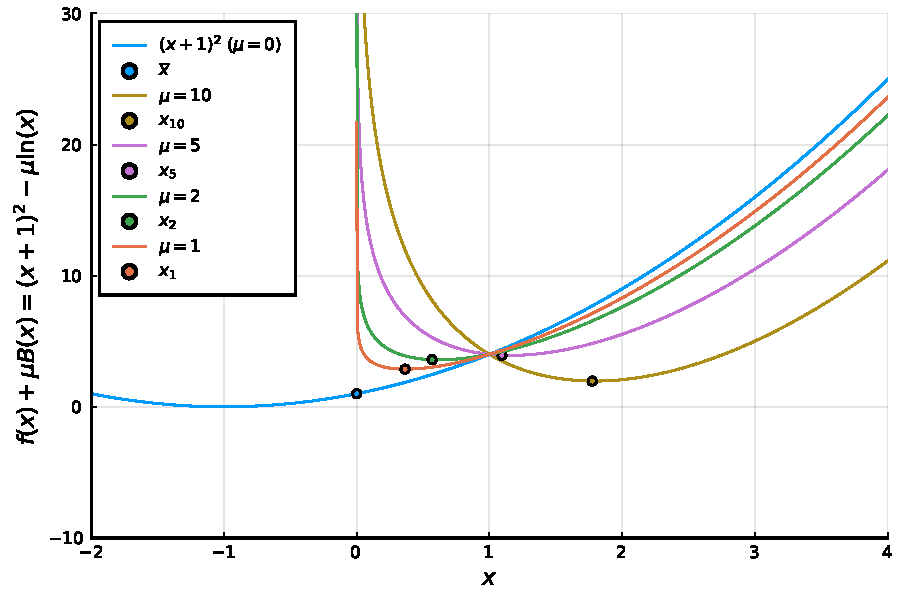
\includegraphics[width=0.8\textwidth]{part_1/chapter_7/figures/ex-barrier.pdf}
	\caption{The optimal values of $P_\mu$ for different values of $\mu$. Notice the trajectory formed by the points $x^*(\mu)$ as $\mu \to 0$.} \label{p1c7:fig:example-barrier} 	
\end{figure}


\subsubsection{The notion of interiority}

There is an interesting link between barrier methods and the notion of interior points, which is in a way, the reason why the two ideas are equivalent. Before we show they are indeed equivalent, let us explore this notion of interiority.

For a large enough $\mu$, the solution of the barrier problem $P_\mu$ is close to the \emph{analytic centre} of the polyhedral feasibility set. The analytic centre of a polyhedral set is	the point at which the distance to all of the hyperplanes forming the set is maximal. More precisely, consider the polyhedral set $S = \braces{x \in \reals^n : Ax \leq b} $. The analytic centre of $S$ is given by the optimal solution $x^*$ of the following problem
	%
	\begin{align*}
		\maxi_x & \prod_{i=1}^m (b_i - a_i ^\top x) \\
		\st & x \in X, 	
	\end{align*}
	%	 
	Notice that we obtain an equivalent problem, that is, a problem would return the same optimal solution $x^*$, if we take the logarithm of the objective function, this would lead to
	%
	\begin{align*}
		\mini_x & \sum_{i=1}^m -\ln(b_i - a_i ^\top x) \\
		\st & x \in S. 	
	\end{align*}
	%
	This allows us to infer something about the behaviour of the barrier method. For larger values of $\mu$, the optimal solution of $x^*(\mu)$ will lie close to the analytical centre of the feasible region. On the other hand, as $\mu$ diminishes, the ``pull'' towards the centre slowly decays whilst the pull caused by the objective function (that is, by its gradient $-\nabla f(x)$) slowly becomes more prevalent and steers the solution towards $x^*$.


\section{Barrier methods for linear programming problems}

Let us consider again our linear programming problem in standard form 
	$$
	(P) : \mini\braces{c^\top x : Ax = b, x \ge 0}
	$$ 
	to which we want to devise a barrier problem. The barrier problem for $P$ is
	%
	\begin{align*}
		(P_\mu) :~ \mini \ &c^\top x  - \mu\sum_{i=1}^n \ln(x_j)\\
		\st &Ax = b \ \ ( \text{and} \ \ x > 0). 
	\end{align*}
	
By looking at this formulation, and relating to the previous discussion, a barrier method for a linear programming problem operates such that in earlier iterations, or for larger $\mu$ values, the optimal solution $x(\mu)^*$ of $P_\mu$ tends to be pushed towards the centre of the feasible region, where $x >0$. As $\mu \to 0$, the influence of $c^\top x$ gradually takes over, steering the solution towards the optimal $x^*$ of $P$. 

Now to the most remarking result, which ties together interior point methods and barrier methods for linear programming problems. If we derive the Karush-Kuhn-Tucker optimality conditions for $P_\mu$, we obtain the following set of conditions
	% 
	\begin{align*}
		&Ax = b, \ x > 0\\ 
		&A^\top p = c - \mu\left(\frac{1}{x_1},\dots,\frac{1}{x_n}\right).
	\end{align*}
	% 
	Using the same notation as before (i.e., defining $X$ and $U$), these can be equivalently rewritten as 
		\begin{align*}
			&Ax = b, \ x > 0 \\ 
			&A^\top p + u = c \\ 
			&u = \mu X^{-1}e ~\Rightarrow~ XUe = \mu e, 
		\end{align*}
	which are exactly \eqref{p1c7:eq:optimality_conditions_matrix_primal}-\eqref{p1c7:eq:optimality_conditions_matrix_relaxed_cc}. Thus, it becomes clear that relaxing the complementarity conditions in the way that we have done before is equivalent to imposing logarithmic barriers to the nonnegativity constraints of $x$. 
	
There are many important consequences for the analysis of the method once this link is established. One immediate consequence relates to the convergence of the method, meaning that as primal and dual feasibility conditions are satisfied throughout the iterations of the method, as $\mu \to 0$, complementarity conditions are satisfied in the limit, thus converging to the solution of the original linear programming $P$. 

Indeed, the trajectory formed by successive solutions $\braces{(x(\mu), p(\mu), u(\mu))_{k=1,2,\dots}}$ is called the \emph{central path}, which is a consequence of the interiority forced by the barrier function. This property is the reason why barrier methods are sometimes called ``path-following'' methods.

It is interesting to also notice the information encoded in \eqref{p1c7:eq:optimality_conditions_matrix_relaxed_cc}. First, notice from \eqref{p1c7:eq:optimality_conditions_matrix_relaxed_dual} that 
	%
	\begin{align*}
		& A^\top p + u = c \Leftrightarrow \\	
		& p^\top (A^x) + u^\top x = c^\top x  \Leftrightarrow  \\
		& u^\top x = c^\top x - p^\top b.
	\end{align*}
	%
	That is, $u^\top x$ provides us with an estimate of the current \emph{duality gap}, which can be used to estimate how far we are from the optimal solution. Moreover, notice that
	$$
	u^\top x = \sum_{i =1}^n u(\mu)_i x(\mu)_i = n\mu 
	$$
	%
	meaning that the term $\mu$ indicates the average amount of violation per $x$ and $u$ variable pairs at $(x^k, p^k, u^k)$. 


\subsubsection{A practical implementation of the barrier method}

The version of the barrier method most often used has a few additional ideas incorporated into the algorithm. One of the main ideas consists of the use of single Newton steps for each value of $\mu$. That effectively means that the iterates do not delineate exactly the central path formed by successively smaller values of $\mu$, but rather follow it only approximately. 

More precisely, assume we start with $\mu_k > 0$ and a $(x^k, p^k, u^k)$ close to $(x(\mu)^k, p(\mu)^k, u(\mu)^k)$. Then, for a small $\beta \in (0,1)$, a Newton step with $\mu_{k+1} = \beta \mu_k$ leads to $(x^{k+1}, p^{k+1}, u^{k+1})$ close to $x(\mu)^{k+1}, p(\mu)^{k+1}, u(\mu)^{k+1}$. Now, to be more precise in terms of what is meant by close, we must refer to the notion of \emph{central paths neighbourhoods}.

A common neighbourhood often used in convergence analysis of the barrier method is
	%
	\begin{equation*}
		N_{\mu_k}(\alpha) =  \braces{(x, p, u) : \|X  U e - \mu_k e \|_2 \leq \alpha \mu_k},
	\end{equation*} 
	%
	which essentially consists of a bound on the difference between the expected value of the complementarity condition violation $\mu$ and that observed by the current solution $(x^k, p^k, u^k)$. The parameter $\alpha \in (0,1]$ is an arbitrary scalar that dictates the amount of such difference tolerated and effectively controls how wide the neighbourhood is. Then, by setting values for $\beta$ and $\alpha$ that satisfy $\beta = 1 - \frac{\sigma}{\sqrt{n}}$ for some $\sigma \in (0,1)$ (e.g., $\alpha = \sigma = 0.1)$, one can guarantee that the complementarity violation of the next iteration to be bounded such that $(x^{k+1}, p^{k+1}, u^{k+1}) \in N_{\mu_{k+1}}(\alpha)$ \cite{gondzio2012interior}. Figure XX illustrate this idea, depicting two successive iterates of the method remaining within the shrinking neighbourhoods $N_{\mu_k}(\alpha)$. 
	
	\begin{figure}
			\begin{tikzpicture}
				\node at (0,0) {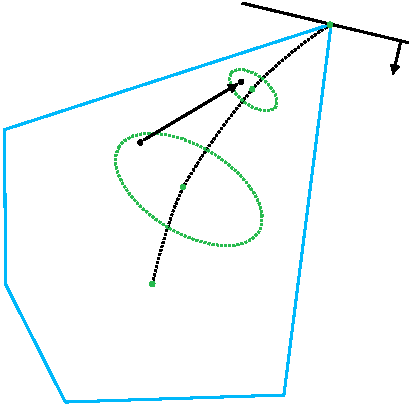
\includegraphics{part_1/chapter_7/figures/central_path_lp-eps-converted-to.pdf}};
		%		\draw[help lines] (-4,-4) grid (4,4);
				\node[below] at (-0.4,-1.2) {$x_{+\infty}$};
				\node[right] at (-0.4,0.2) {$x_{\mu_k}$};		
				\node[below] at (1.3,2.1) {$x_{\mu_{k+1}}$};
				\node[right] at (-1.2,0.9) {$x^k$};
				\node[above] at (0.8,2.05) {$x^{k+1}$};
				\node[below] at (3.5,2.6) {$c$};
				\node[below] at (0.4,-0.6) {$N_{\mu_1}(\alpha)$};
				\node[below] at (1.1,1.7) {$N_{\mu_2}(\alpha)$};	
			\end{tikzpicture}	
			\caption{An illustrative representation of the central path and how the method follows it approximately}
		
	\end{figure}
	
Another important aspect related to the method consists of the feasibility requirements of each step. Current implementations of the method can be shown to converge under particular conditions even if the feasibility requirements are eased in the Newton system. In particular, it can be shown that the Newton direction is also such that the amount of infeasibility in the system decreases as the algorithm progresses. 
	
The infeasible version of the algorithm is such that, the perturbed system
	%
	\begin{equation*} 	
		\begin{bmatrix} A  & 0 & 0 \\ 
						0  & A^\top & I \\ 
						U^k  & 0 & X^k 
		\end{bmatrix} 
		\begin{bmatrix} d_x^{k+1} \\ 
					    d_p^{k+1} \\ 
					    d_u^{k+1} 
		\end{bmatrix} =  
		\begin{bmatrix} 0 \\ 
						0 \\ 
						\mu_{k+1} e - X^k U^k e 
		\end{bmatrix}. 
	\end{equation*} 
	%
	becomes 
	%
	\begin{equation}\label{p1c7:eq:infeasible_perturbed_system}
	\begin{bmatrix} A  & 0 & 0 \\ 
					0  & A^\top & I \\ 
					U^k & 0 & X^k 
	\end{bmatrix} 
	\begin{bmatrix}d_x^{k+1} \\ 
				   d_p^{k+1} \\ 
				   d_u^{k+1} 
	\end{bmatrix} = - 
	\begin{bmatrix} Ax^k - b \\ A^\top p^k + u^k - c \\ X^k U^ke -\mu_{k+1}e \end{bmatrix}. 
	\end{equation}
	where $\mu_{k+1} = \beta\mu_k$.

The primal residual $r_p(x) = Ax - b$ and dual residual $r_d(p,u) = A^\top p + u - c$ allow the method to iterate through solutions $(x^k, p^k, u^k)$ that do not satisfy primal and/ or dual feasibility. A caveat thought is that the convergence analysis of this variant is more involved and requires additional assumptions on the parametrisation of the algorithm for convergence. 

To see how the residuals decay a teach iteration, notice the following. Let $r(w) = r(x,p,u) = (r_p(x), r_d(p,u))$. The optimality conditions \eqref{p1c7:eq:optimality_conditions_primal}-\eqref{p1c7:eq:optimality_conditions_cc} require the residuals to vanish, that is, $r(w) = 0$. Now, let us consider the first-order approximation for $r$ at $w^k$ for a Newton step $d_w$. This amounts to the following:
	$$
	r(w^k + d_w) \approx r(w^k) + Dr(w^k)d_w,
	$$
	where $Dr(w^k)$ is the Jacobian of $r$ evaluated at $w^k$. One can notice that, in this notation, the solution $d_w^{k+1}$ to \eqref{p1c7:eq:infeasible_perturbed_system} is such that 
		$$
		Dr(w^k) d_w^{k+1} = -r(w^k).
		$$

Now, let us consider the directional derivative of the norm of the updated residues in the direction $d_w^{k+1}$. That leads to the following conclusion
	%
	\begin{equation*}
		\frac{d}{dt} \big\| r(w^k + td_w^{k+1}) \big\|_2^2 \Big|_{t = 0} = 2r(w^k)^\top Dr(w^k)d_w^{k+1} = -2 \| r(w^k) \|_2^2 < 0.
	\end{equation*}
	%
	This shows that the direction $d_w^{k+1}$ is a descent direction for the norm of the residues at $w^k$ which leads to their eventual vanishing.	
	
We are finally ready to pose the pseudocode of a working version of the barrier method, which is displayed in Algorithm \ref{p1c7:alg:barrier_method}.
	%
	\captionsetup[algorithm]{font=footnotesize}
	\begin{algorithm}[H]
	\caption{Barrier method for LP} \label{p1c7:alg:barrier_method}
	\begin{algorithmic}[1] 
	\State {\bf initialise.} \text{(primal-dual feasible)} $(x^0, p^0, u^0)$, $\epsilon > 0$, $\mu_0 = \mu_1>0$, $\beta \in (0,1)$, $k = 0$. 
	\While {$n \mu_k > \epsilon$}
	    \State compute $d^{k+1} = (d_x^{k+1}, d_p^{k+1}, d_u^{k+1})$ using \eqref{p1c7:eq:infeasible_perturbed_system} 
	    \State compute appropriate step size $\theta^{k+1} = (\theta_p^{k+1}, \theta_d^{k+1}$)
	    \State $(x^{k+1}, p^{k+1}, u^{k+1}) = (x^k, p^k, u^k) + \theta^{k+1}d^{k+1}$
	    \State $k = k+1$
	    \State $\mu_{k+1} = \beta\mu_k$
	\EndWhile
	\State {\bf return} $w^k$.
	\end{algorithmic} 
	\end{algorithm}
	
Some final remarks are worth making. Barrier methods are perhaps the only class of methods that are known for being strong contenders to the dominance of simplex method-based approaches for linear programming problems. This stems from both a theoretical and an experimental perspective. The analysis available in \cite{gondzio2012interior} shows that the number of iterations of the barrier method, for suitable parameterisation, is $O(\sqrt{n}\ln(1/\epsilon))$, whilst, for the simplex method, a similar analysis would bound the number of iterations to be of the order $O(2^n)$. A conclusion stemming from these results would be that barrier methods, being polynomial complexity algorithms, should outperform the simplex method.

But in practice, this is not necessarily the case. Despite its complexity analysis, the simplex method in practice often requires $O(m)$ iterations (i.e., a typically modest multiple of $m$), where $m$ is the number of columns in the basis. On the other hand, practical observation has shown barrier methods to typically require $\sqrt{n}$ iterations or less and appear to be somewhat insensitive to growth in the number of variables further to a certain point. On the other hand, one iteration of the simplex method is rather inexpensive from a computational standpoint, while one iteration of a barrier method is a potentially computationally demanding operation (as it requires the solution of a large linear system of equations).

In general, simplex-method-based solvers are faster on problems of small to medium dimensions, while barrier methods are competitive, and often faster, on large problems. However, this is not a rule, as the performance is dependent on the structure of the particular application. In the end, it all boils down to how effectively the underlying liner system solver can exploit particular structural features employing dedicated numerical algebra methods (e.g., sparsity and the use of Cholesky decomposition combined with triangular solves).

Moreover, barrier methods are generally not able to take full advantage of any prior knowledge about the solution, such as an estimate of the solution itself or some suboptimal basis. Hence, barrier methods are less useful than simplex approaches in situations in which ``warm-start'' information is available. One situation of this type involves branch-and-bound algorithms for solving integer programs, where each node in the branch-and-bound tree requires the solution of a linear program that differs only slightly from one already solved in the parent node. In other situations, we may wish to solve a sequence of linear programs in which the data is perturbed slightly to investigate the sensitivity of the solutions to various perturbations, or in which we approximate a non-linear optimisation problem by a sequence of linear programs. In none of the above scenarios barrier methods can be used as efficiently as the simplex method (dual or primal, depending on the context).

\vfill
\pagebreak	

\section{Exercises}


